%% V1.0
%% by Christopher Leith, udacl@cielsystems.com
%% This is a template for Udacity projects using IEEEtran.cls

\documentclass[10pt,journal,compsoc]{IEEEtran}

\usepackage[pdftex]{graphicx}    
\usepackage{cite}
\hyphenation{op-tical net-works semi-conduc-tor}

\begin{document}

\title{Robotic Inference}

\author{Christopher Leith}

\markboth{Inference project, Robotic Nanodegree, Udacity, NVidia Digits}%
{}
\IEEEtitleabstractindextext{%

\begin{abstract}
Robotic applications requiring object recognition and classification are becoming commonplace. Two different recognition applications for classifying a common object in an image using neural networks are discussed and network training using the NVidia Digits workflow is demonstrated for training 2 common networks: AlexNet and GoogLeNet
\end{abstract}

% Note that keywords are not normally used for peerreview papers.
\begin{IEEEkeywords}
Robot, Mobile Robot, Udacity, Neural Network, NVidia Digits.
\end{IEEEkeywords}}


\maketitle
\IEEEdisplaynontitleabstractindextext
\IEEEpeerreviewmaketitle
\section{Introduction}
\label{sec:introduction}

\IEEEPARstart{T}{he}. 
Robotic automation of industrial processes such as assembly lines or mail sorting have been common for decades. Now mobile robotic systems are also becoming commonplace and similar image classification tasks will be useful on these platforms. The ability to deploy trained classification neural networks that will operate on these less performant, general purpose systems will be very useful and valuable. In this paper 2 such classification networks will be discussed: A Classifier to distinguish candy boxes from bottles and a classifier to distinguish 2 kinds of coins, U.S. quarters vs U.S. pennies. Even these very simple demonstration projects could find realistic use cases for a 'personal robot' that could help with recycling or with segregating coins for putting into 'coin rolls'. And of course there are an unlimited number of applications like this that could be useful for personal or business assistant robots. The ability to quickly create and deploy a classifier for new, general purpose segregation tasks to be performed by a personal robot are endless. This demonstration project illustrates how simple it is to create the classifier networks that could then be deployed.

If you have any papers / sites you have referenced for your idea, please make sure to cite them.

\section{Background / Formulation}
The topic of deep learning and convolutional neural networks is vast. Designing neural networks using popular libraries such as google TensorFlow can be too complicated for inexperienced developers. Fortunately there exist already many effective, CNN designs that are available for free use. The NVidia Digits application provides 3 well known CNNs: LeNet, AlexNet, and GoogLeNet ready for immediate use. These CNNs have different strengths and weakness.

\subsection{Task1 Bottle vs Candy Box}
The premise for this task is to create a classifier to observe and control an object sorting conveyor belt. A camera is placed above the conveyor and records an image of passing objects. The image is acquired by an NVidia jetson TX2 which classifies the object image and then controls an actuator that routes each object into an appropriate bin. For this project the 2 more advanced CNN networks, AlexNet and GoogLeNet were chosen to assess which would perform better for the requirements. The more primitive LeNet was not tried, in part because the complexity of the images appeared to be too complicated for compression into the 28x28 pixel greyscale images required by this network.
Several backpropagation optimizers were tried experimentally, but due to VM timeout these models were lost. In the submission the Stochastic Descent optimizer was used with thee Alex net and the default Adam optimizer was used with the GoogLeNet becasue these were found to meet the specifications empirically.

\subsection{Task2 Quarter vs Penny}
The premise for the second task is very similar to Task1. Given a coin from a mix of pennies and quarters create a classifier network that can distinguish them. Since the hypothetical use case was a mobile robot instead of a conveyor the images were not taken from a fixed distance. Furthermore the coins have 2 sides and a variety of actual engraved detail and the mobile robot would encounter all of those variations, all variations were included in the dataset. Based on the results from Task1 the GoogLeNet CNN with Stochastic Descent was chosen for this task. Again, LeNet was not considered, especially since the color of the coins were expected to be important for the classsification and LeNet expects greyscale. 

\section{Data Acquisition}
The following subsections detail the data acquisition for the 2 Tasks.

\subsection{Task1 Bottle vs Candy Box}
The image dataset for this task was provided by Udacity. It was automatically provisioned into the workwpace VM into 
/data/P1\_data/directory.
All of the files were color 256x256 pixel color png files, and since this is the expected format for the selected networks, no image preprocessing was needed.


\begin{table}[h]
\caption{Task1 training images}
\label{Task1 training images}
\begin{center}
\begin{tabular}{|c||c|}
\hline
Class Directory & Num Images\\
\hline
/data/P1\_data/Bottle & 3426\\
/data/P1\_data/Candy\_box & 1871\\
/data/P1\_data/Nothing & 2273 \\
\hline
\end{tabular}
\end{center}
\end{table}

\subsection{Task2 Quarter vs Penny}

\subsubsection{Photography}
The coin images dataset was obtained using 4 iphones of different models. Coins, first quarter heads then quarter tails then pennies heads then pennies tails. were layed in a 11x6 grid on a flat white paper surface. The surface was illuminated from several directions from incandescent, halogen and reflected sunlight. Child labor was then employed to take a pictures of each coin with each phone. The orientation of the photos were random. However the photographers were instructed to keep the lens approximately 15-20 centimeters directly above the coin. This was found to be a good height for the autofocus to converge quickly. The cameras were also zoomed in so that the coin image would record "pretty big" and photographers were asked to insure that more than half of the coin was recorded in the image. All photos used square photo setting with flash and High Dynamic Range disabled.

All photos from each phone were then transferred to a computer and combined. Heads and tails were placed in the same class together. In this transfer process it seems that somee photos were lost, but enough were present to run the training.

\subsubsection{Image Culling}
Before further processing the images were reviewed for quality. Images that were terribly out of focus or mostly out of frame were deleted form the dataset. Images that had more than 2 coins visible were deleted. After the culling the total number of training images was 

\begin{table}[h]
\caption{Task2 training images}
\label{Task2 training images}
\begin{center}
\begin{tabular}{|c||c|}
\hline
Class Directory & Num Images\\
\hline
Pennies & 460\\
Quarters & 429\\
\hline
\end{tabular}
\end{center}
\end{table}

\subsubsection{Post Processing}
The raw photos were color JPG images and varied in resolution either
2448x2448 or 3024x3024 depending on the model of the phone. In order to keep the data set small and easy to transfer all images were resized to 256x256 pixels using a python script, ./src/resizephotos.py.

\subsubsection{Transfer}
The final training photos were commited to a github repository

github.com/cielsys/RoboND2\_Proj1\_Inference

into directory ./Assets/raw\_resized\_256x256
and subdirectories
1\_penny/ and 2\_quarter/

These were then retrieved into the workspace VM for manipulation by the DIGITS application.

\section{Results}
The following subsections detail the results for the 2 Tasks.

\subsection{Task1 Bottle vs Candy Box}
Both GoogLeNet and AlexNet were able to hit the performance goals of 75\% accuracy in under 10mSec.

\subsubsection{Task1 AlexNet}
Fig 1 shows that AlexNet classifications took approximately 4mS with an average accuracy of 75.4\%. It is evident from the validation training accuracy of near 100\% that 30 epochs of training was too much and that overfitting was likely for this model. 

\begin{figure}[h]
      \centering
      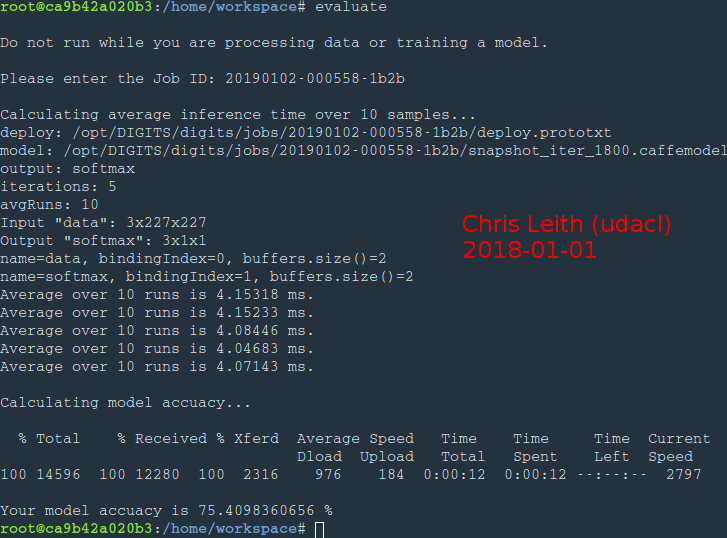
\includegraphics[width=\linewidth]{Assets/screenshots/P1_Evaluate_Alex01_x1.png}
      \caption{Task1 Evaluate AlexNet }
      \label{fig:Task1 Evaluate AlexNet }
\end{figure}


\begin{figure}[h]
      \centering
      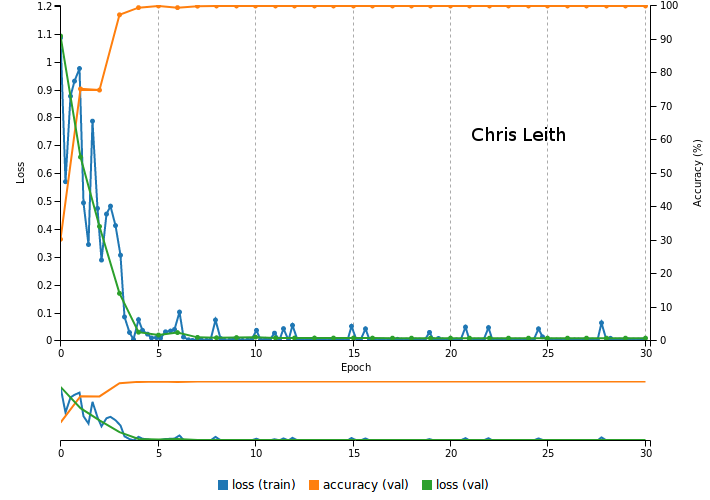
\includegraphics[width=\linewidth]{Assets/screenshots/Screenshot_2019-01-01_P1_alex1_30E.png}
      \caption{Task1 Training AlexNet}
      \label{fig:Task1 Training AlexNet}
\end{figure}

\subsubsection{Task1 GoogLeNet}
Fig 4 shows that GoogLeNet classifications took slightly longer than the AlexNet, about 5.5mS, but still within the 10mS goal with an identical accuracy.

\begin{figure}[h]
      \centering
      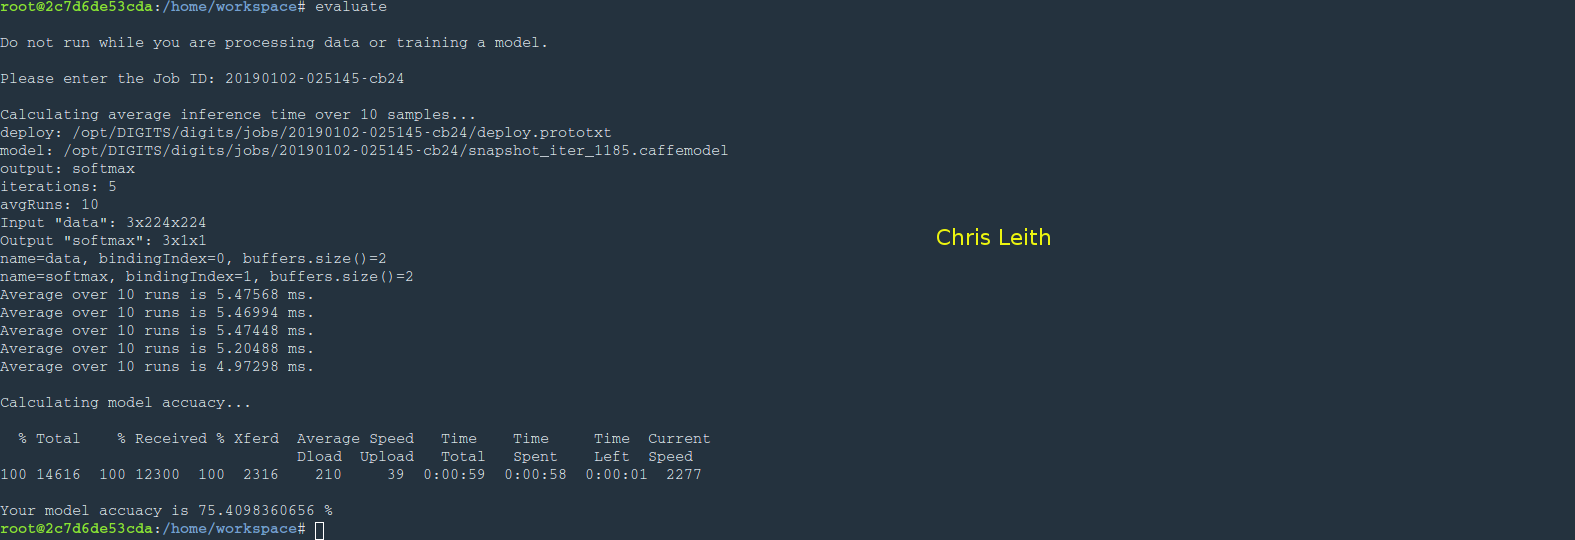
\includegraphics[width=\linewidth]{Assets/screenshots/Screenshot_2019-01-01_P2_google03_adam_E5_accuracy.png}
      \caption{Task1 Evaluate GoogLeNet }
      \label{fig:Task1 Evaluate GoogLeNet}
\end{figure}


\begin{figure}[h]
      \centering
      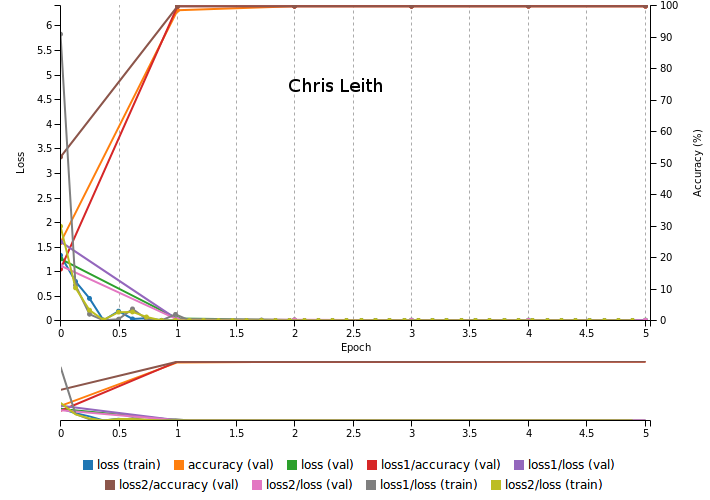
\includegraphics[width=\linewidth]{Assets/screenshots/Screenshot_2019-01-01_P2_google03_adam_E5.png}
      \caption{Task1 Training GoogLeNet }
      \label{fig:Task1 Training GoogLeNet}
\end{figure}


\subsection{Task2 Quarter vs Penny}
Only the GoogLeNet was used for the coin classification. Fig 6 shows the validation accuracy approaching 90\% and a spot check of 10 random coins also shows 9 out of 10 correct classifications (Fig ~\ref{fig:Task2 Correctly Classified}) and 1 incorrect classification (Fig ~\ref{fig:Task2 Incorrectly Classified} )

\begin{figure}[h]
      \centering
      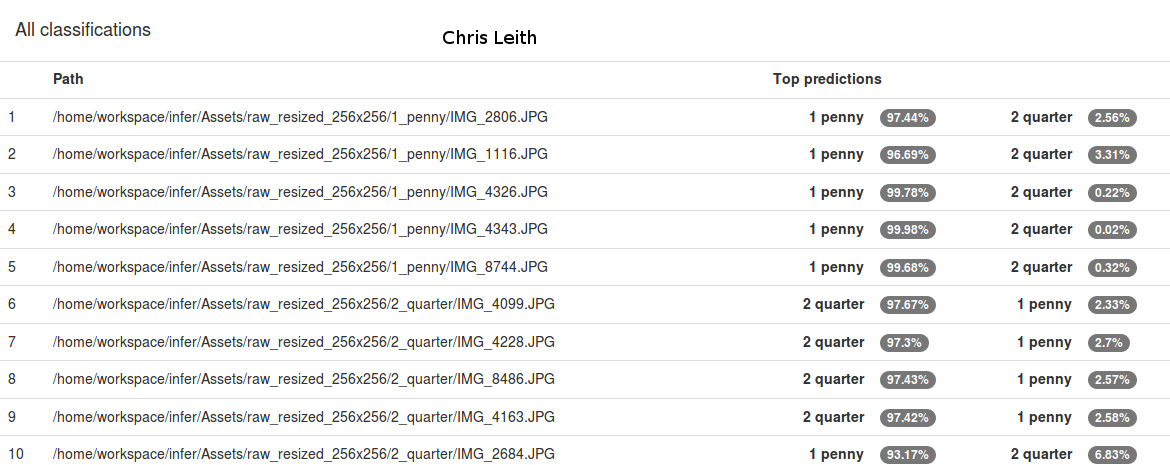
\includegraphics[width=\linewidth]{Assets/screenshots/Screenshot_2019-01-01_coins1_eval_google01.png}
      \caption{Task2 Evaluate GoogLeNet }
      \label{fig:Task2 Evaluate GoogLeNet}
\end{figure}


\begin{figure}[h]
      \centering
      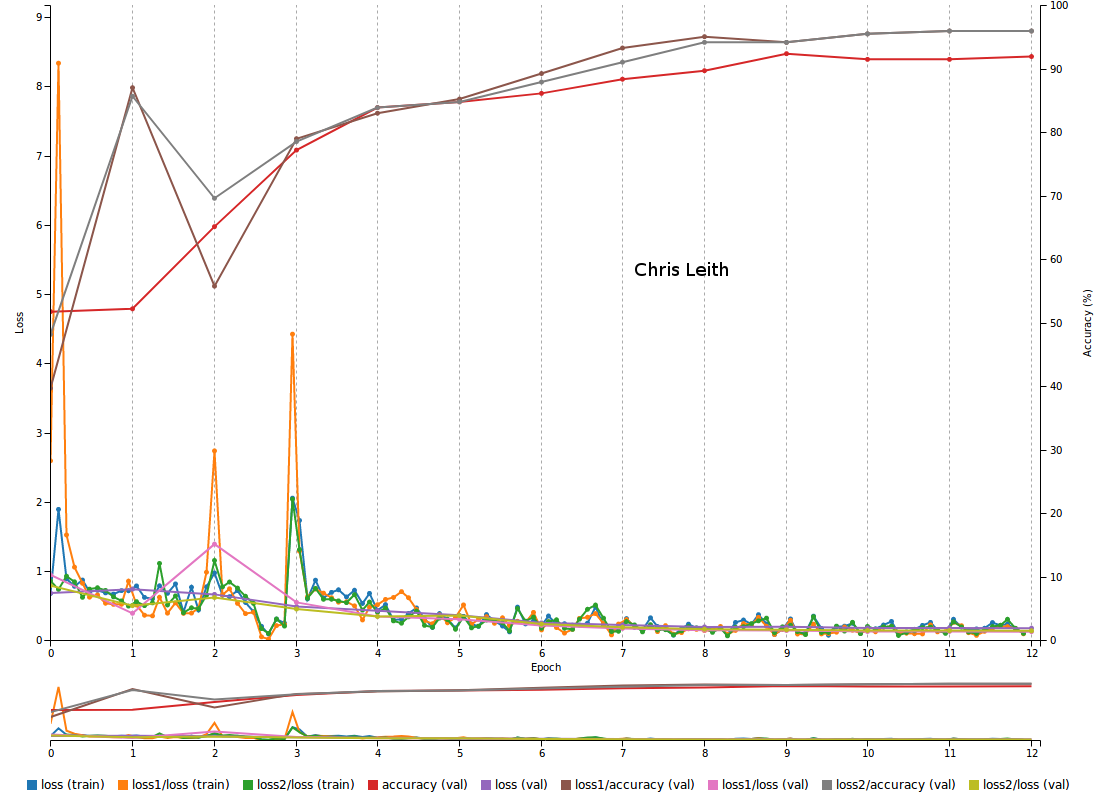
\includegraphics[width=\linewidth]{Assets/screenshots/Screenshot_2019-01-01_coins1_train_google01.png}
      \caption{Task2 Training GoogLeNet }
      \label{fig:Task2 Training GoogLeNet}
\end{figure}


\begin{figure}[h]
      \centering
      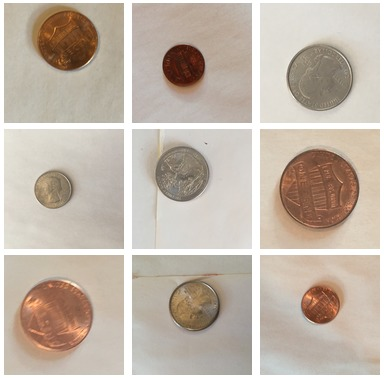
\includegraphics[width=\linewidth]{Assets/testset2_10/report/correctcoins.JPG}
      \caption{Task2 Correctly Classified }
      \label{fig:Task2 Correctly Classified}
\end{figure}


\begin{figure}[h]
      \centering
      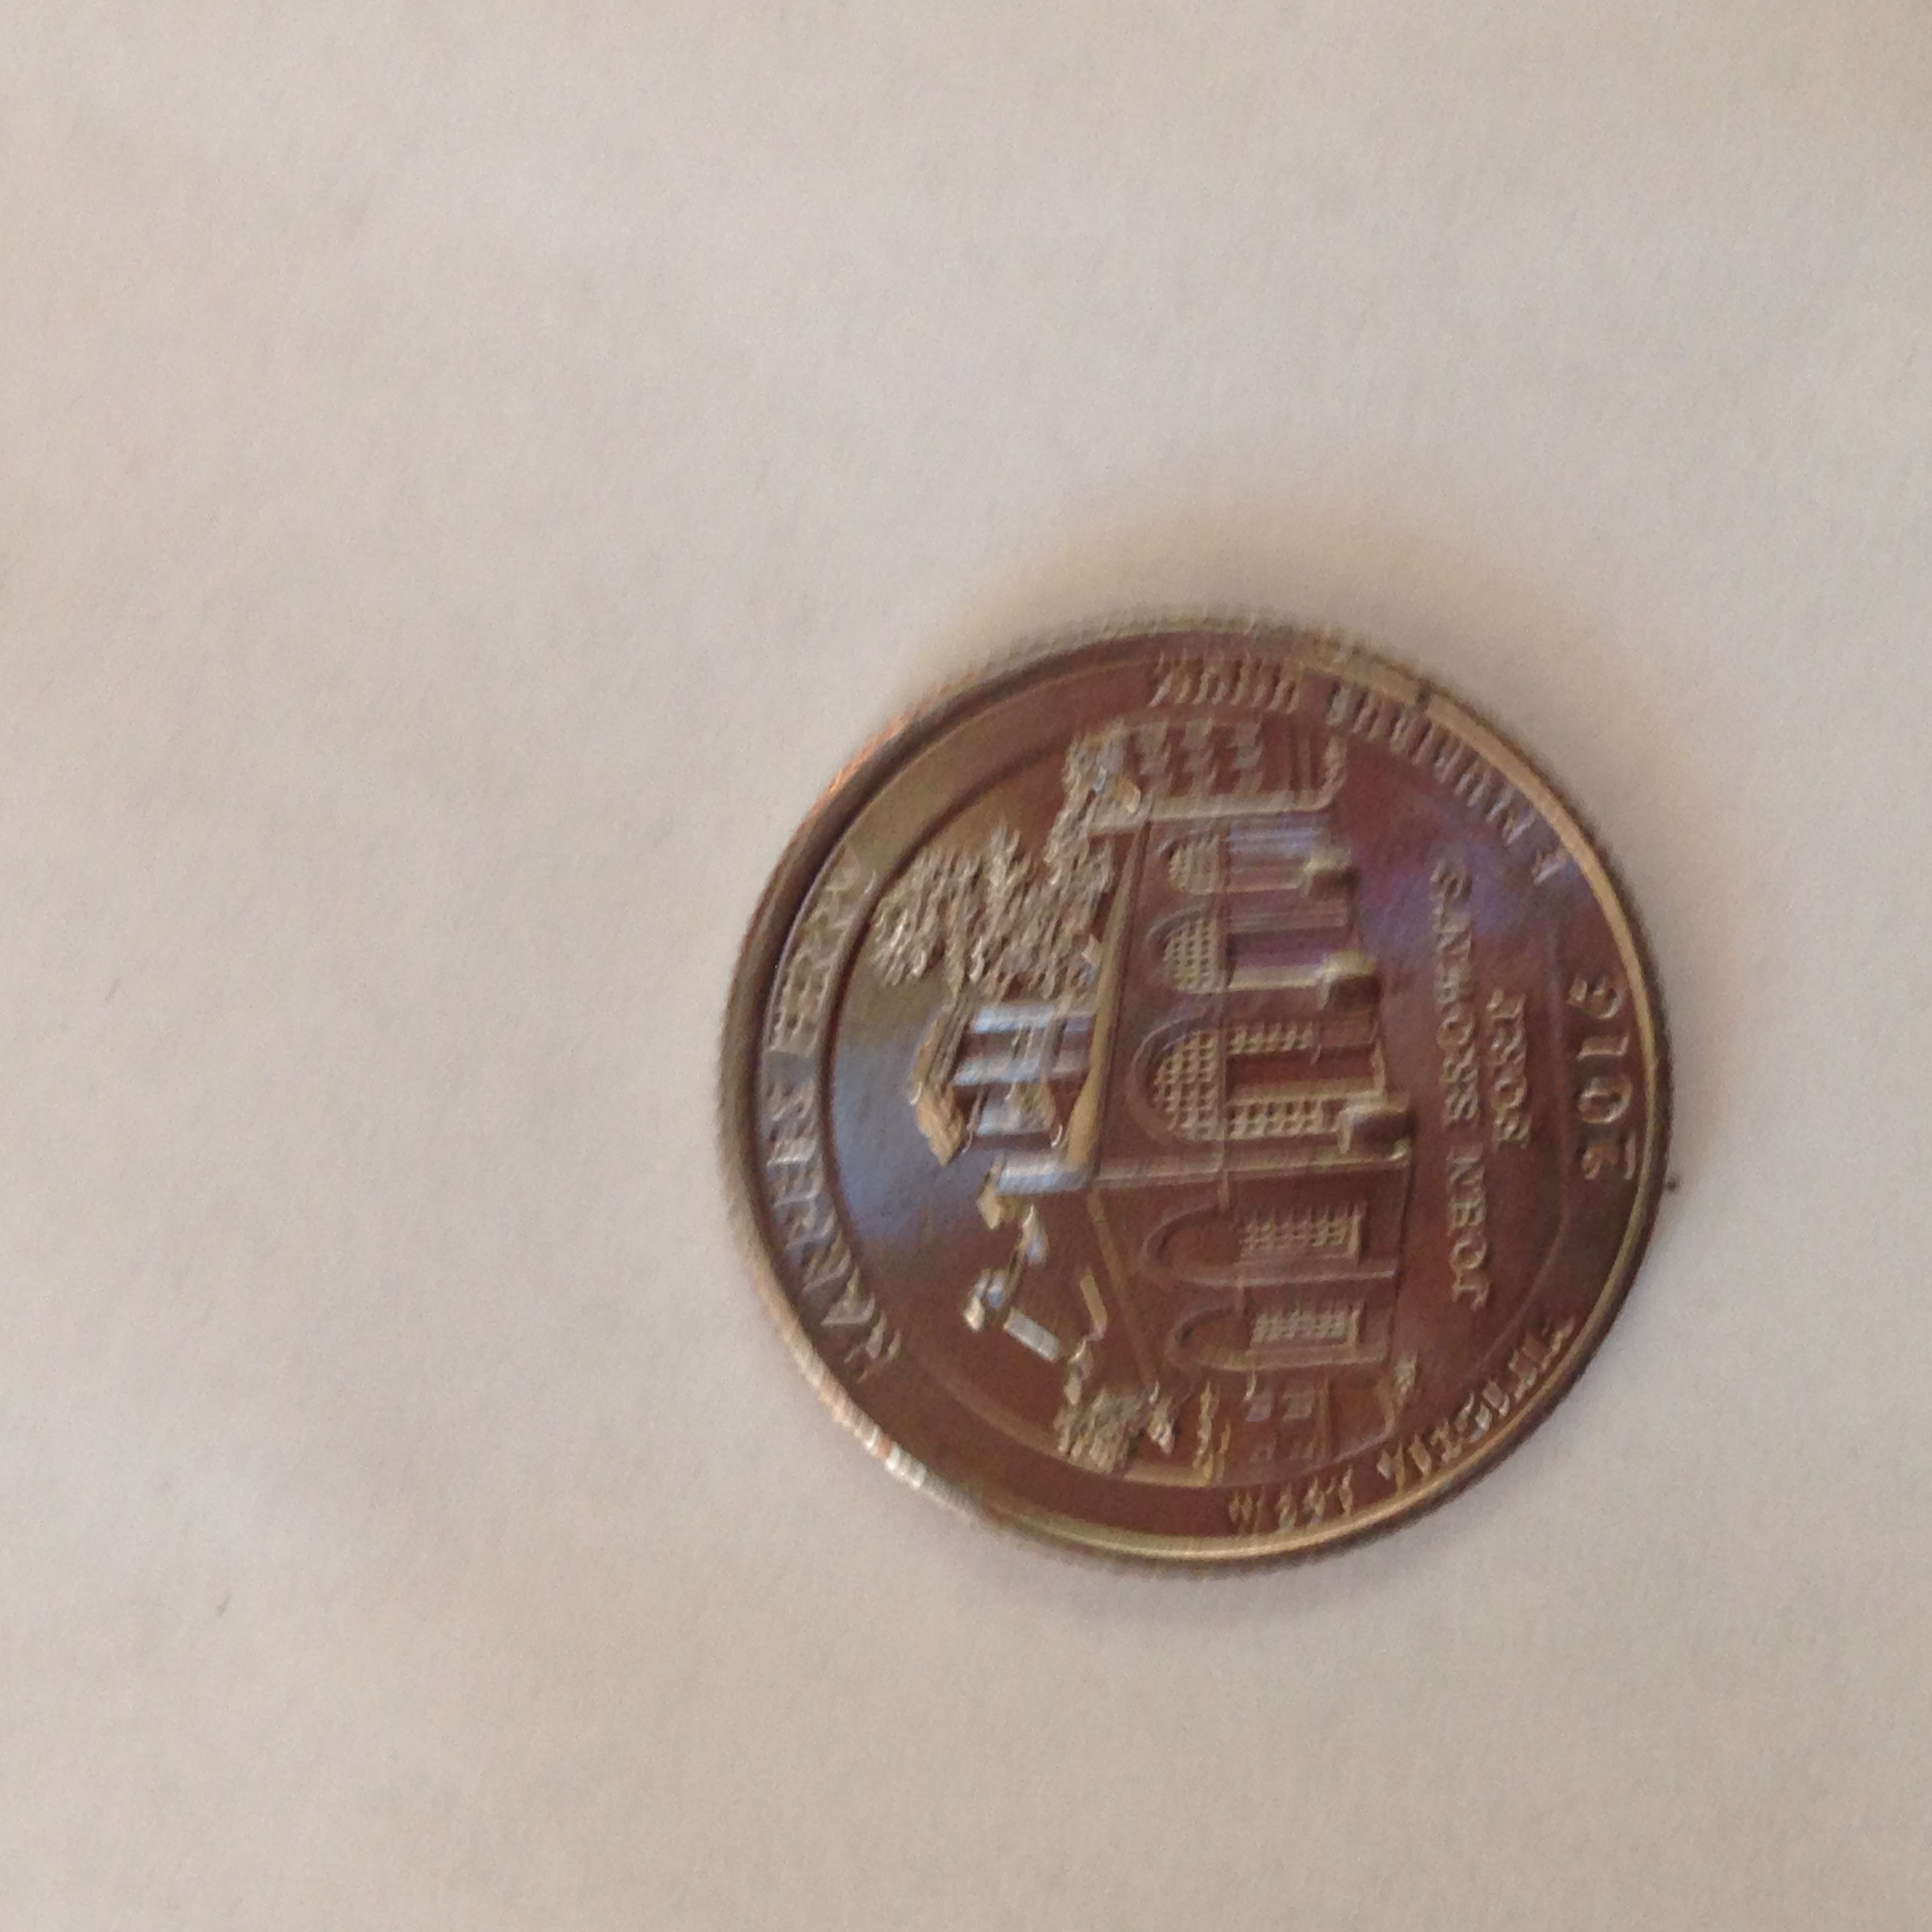
\includegraphics[width=\linewidth]{Assets/testset2_10/report/IMG_2684.JPG}
      \caption{Task2 Incorrectly Classified }
      \label{fig:Task2 Incorrectly Classified}
\end{figure}


\begin{figure}[h]
      \centering
      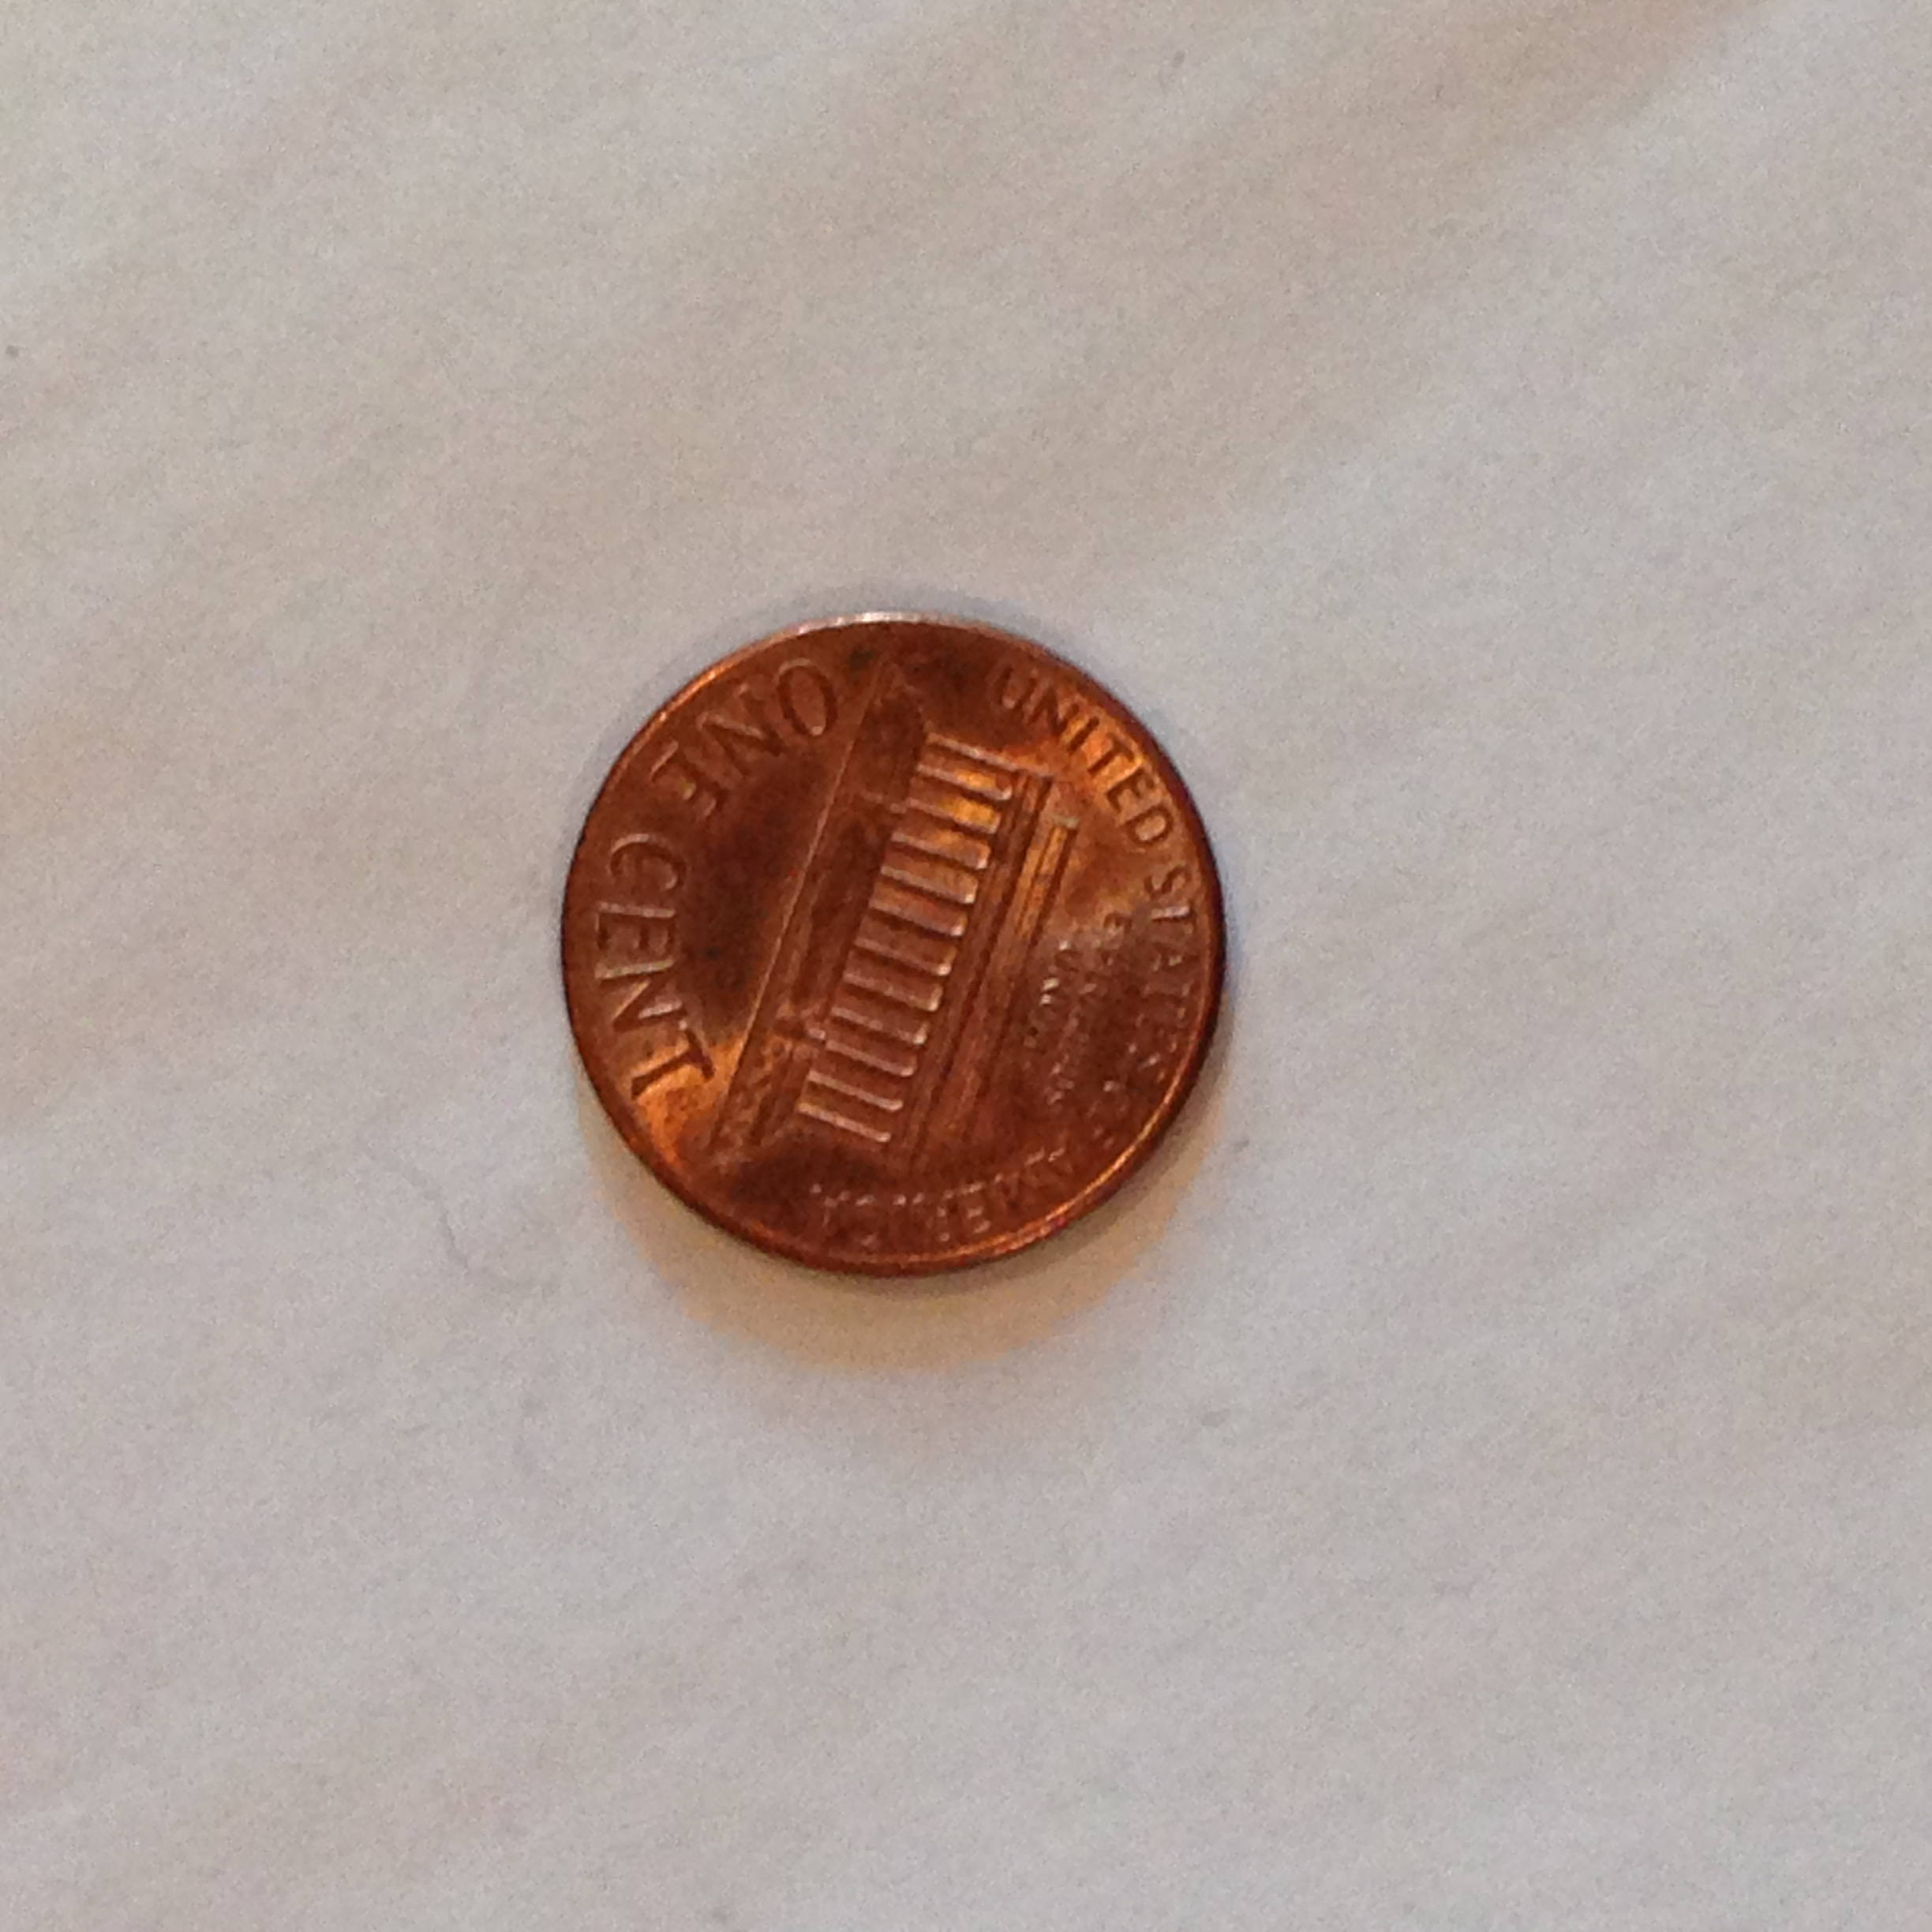
\includegraphics[width=\linewidth]{Assets/testset2_10/report/IMG_2835.JPG}
      \caption{Task2 Standard Penny }
      \label{fig:Task2 Standard Penny}
\end{figure}




\section{Discussion}
Both classification tasks were successful using mostly default values for the selected network models.

\subsection{Task1 Bottle vs Candy Box}
Since the classification network met the given requirements of this contrived task of 75\% accuracy in under 10mS it is deemed successful. Would this performance be succesful in a real world application? It entirely depends on the actual application. In many assembly lines there  are redundancies in place to correct earlier mistakes. In other cases there is simply no great harm in errors occuring. In those scenario classification time is likely the more important criteria. Other applications may place a very high importantance on accuracy, for example if the outputs of the segregation were to be delivered to paying customers.

\subsection{Task2 Quarter vs Penny}
The back sides of quarters and pennies are extremely varied since every state has it's own custom design. Some of the custom quarter back designs (Fig ~\ref{fig:Task2 Incorrectly Classified}) look quite similar to the 'standard' penny back design (~\ref{fig:Task2 Standard Penny}). It is possible this incorrect classification detected the feature of a series of parallel lines. In order to improve accuracy it is anticipated that a larger dataset with equal numbers of each variety of coin would be neccesary for the net to recognize more subtle combinations of features to maintain a high accuracy. Additonally this dataset had all photos from directly above on a uniform background. A mobile robot may not be able to rely on such uniformity so that an even bigger dataset would be needed to get images in the expected variety of the real world. As with Task1 the relative importance of speed versus accuracy would depend entirely on the application. If the coins were to be delivered to smelter for recasting, some error may be acceptable in order to achieve throughput. On the other hand if the segregation were for some monetary application accuracy would be paramount.

\section{Conclusion / Future work}
Training image classification neural networks is now simple enough that any robotic project should be able take advantage of them. NVidia DIGITS was able, with a modest number of training images, to create trained classification networks at the click of a few buttons. The 2 tasks in this report were, however, adimittedly simplistic. A real world robotic system would likley need a wider variety of objects and coins to be useful. And a prototype system for using the nets in real world conditions would no doubt quickly expose the weaknesses of these networks and it would likely need several iterations of dataset generation and network training. Nonetheless it has been shown that creating basic classification Neural Networks is simple and effective.

\end{document}